\documentclass[answers,11pt]{exam}

\makeatletter
\newcommand{\course}[1]{\def\@course{#1}}
\makeatother

\makeatletter
\pagestyle{headandfoot}
\firstpageheader{}{\large \textbf{\@title \ifprintanswers ~-- Solutions \else \fi} \\ \@course}{}
\makeatother


\usepackage{amsmath}
\usepackage{amssymb}
\usepackage{booktabs}
\usepackage{graphicx}
\usepackage{subfig}
\usepackage{hyperref}

\DeclareGraphicsExtensions{.png,.pdf}


\DeclareMathOperator*{\Prob}{P}
\renewcommand{\Pr}{\Prob}
\DeclareMathOperator*{\E}{E}
\DeclareMathOperator*{\var}{var}
\DeclareMathOperator*{\sd}{sd}


\title{The Central Limit Theorem}
\course{STAT-UB.0001 -- Statistics for Business Control}

\begin{document}
\begin{questions}

\fullwidth{\section*{The Central Limit Theorem}}

\question Consider the population of all Fortune 500 CEOs and their salaries.
Suppose that the mean salary (in millions of dollars) is $\mu = 20$, and the
standard deviation of the salaries is $\sigma = 5$.  You sample 50 CEOs and
find their salaries.

\begin{parts}

\part Draw a histogram of what you think the population looks like.

\vspace{\stretch{1}}

\part Let $X$ be the salary of a randomly drawn CEO. Consider $X$ to be a random variable. What is the histogram of $X$? What is its expectation and standard deviation? 
\begin{solution}
$X$ will have the same histogram as the population. $\E [ X]=\mu=20$, and $\sd[X]=\sigma=5$.
\end{solution}

\vspace{\stretch{1}}

\part Consider the sample mean $\bar X$ to be a random variable.  What is the
expectation of $\bar X$?

\begin{solution}
$\E[\bar X] = \mu = 20$.
\end{solution}

\vspace{\stretch{1}}


\part What is the standard deviation of $\bar X$?

\begin{solution}
$\sd[\bar X] = \frac{\sigma}{\sqrt{n}} = \frac{5}{\sqrt{50}} \approx .707$.
\end{solution}

\vspace{\stretch{1}}


\part Draw a picture of what you think the PDF of $\bar X$ looks like.

\begin{solution}
Normal with mean $20$, standard deviation $.707$.
\end{solution}

\vspace{\stretch{1}}

\end{parts}

\newpage


\question You draw a random sample of size $n = 64$ from a population with
mean $\mu = 50$ and standard deviation $\sigma = 16$.  From this, you compute
the sample mean, $\bar X$.

\begin{parts}
\part What are the expectation and standard deviation of $\bar X$?

\begin{solution}
\begin{align*}
  \E[\bar X] &= \mu = 50, \\
  \sd[\bar X] &= \frac{\sigma}{\sqrt{n}} = \frac{16}{\sqrt{64}} = 2.
\end{align*}
\end{solution}

\vspace{\stretch{1}}


\part Approximately what is the probability that the sample mean is above 54?

\begin{solution}
The sample mean has expectation 50 and standard deviation 2.  By the central
limit theorem, the sample mean is approximately normally distributed.  Thus,
by the empirical rule, there is roughly a 2.5\% chance of being above 54
(2 standard deviations above the mean).
\end{solution}

\vspace{\stretch{1}}


\part Do you need any additional assumptions for part (c) to be true?

\begin{solution}
No.  Since the sample size is large ($n \geq 30$), the central limit theorem
applies.
\end{solution}

\vspace{\stretch{1}}

\end{parts}


\question You draw a random sample of size $n = 16$ from a population with
mean $\mu = 100$ and standard deviation $\sigma = 20$.  From this, you compute
the sample mean, $\bar X$.

\begin{parts}
\part What are the expectation and standard deviation of $\bar X$?

\begin{solution}
\begin{align*}
  \E[\bar X] &= \mu = 100, \\
  \sd[\bar X] &= \frac{\sigma}{\sqrt{n}} = \frac{20}{\sqrt{16}} = 5.
\end{align*}
\end{solution}

\vspace{\stretch{1}}


\part Approximately what is the probability that the sample mean is between
95 and 105?

\begin{solution}
The sample mean has expectation 100 and standard deviation 5.  If it is
approximately normal, then we can use the empirical rule to say that there is
a 68\% of being between 95 and 105 (within one standard deviation of its
expectation).
\end{solution}

\vspace{\stretch{1}}


\part Do you need any additional assumptions for part (c) to be true?

\begin{solution}
Yes, we need to assume that the population is normal.  The
sample size is small ($n < 30$), so the central limit theorem may not be in
force.
\end{solution}

\vspace{\stretch{1}}

\end{parts}

  \newpage


  \fullwidth{Here is a histogram of the fares (including tax and tolls) of
    162,997 taxi trips taken within New York City in 2013.}

  \fullwidth{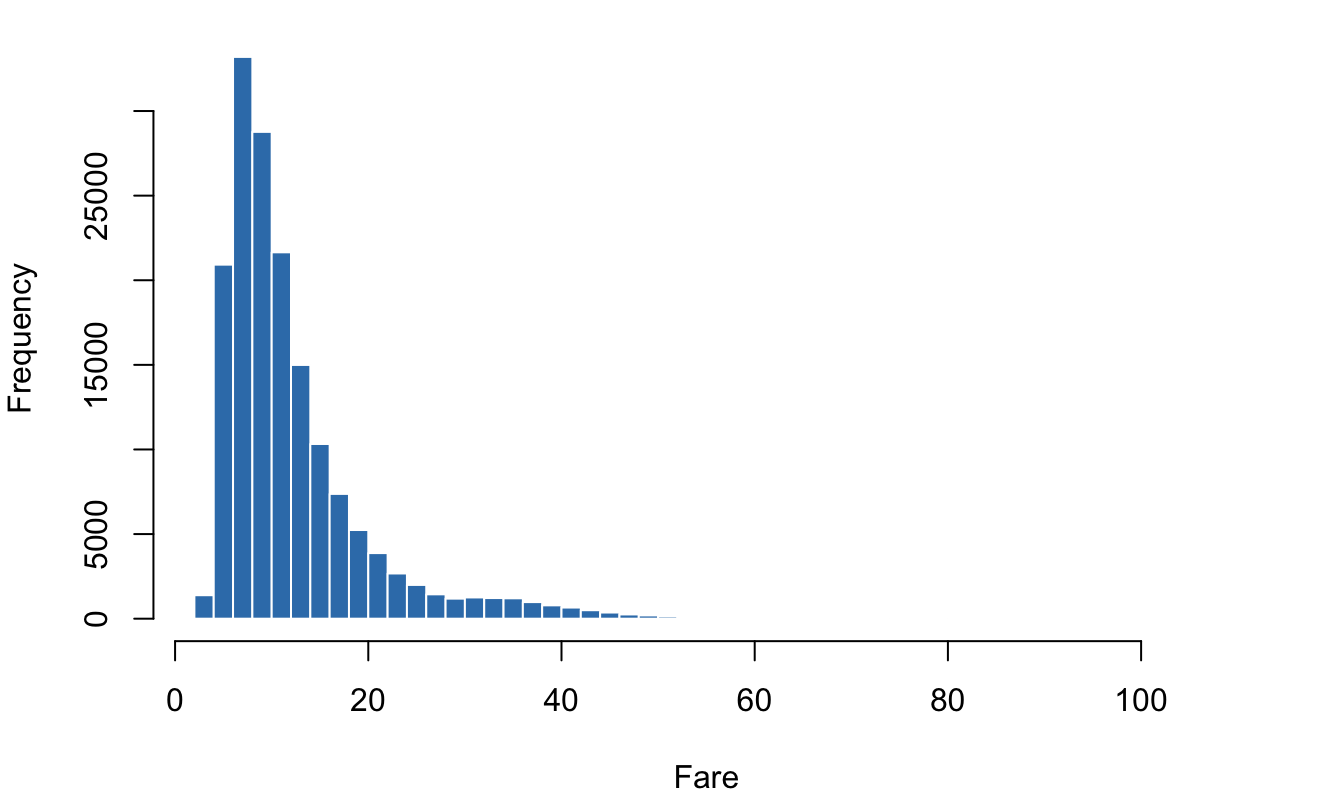
\includegraphics[width=\linewidth]{farehist.png}}

  \fullwidth{The following table displays the trips with the highest and lowest
    fares.}

  \fullwidth{\begin{minipage}{\linewidth}
\centering
%\makebox[6.5in][c]{
%\captionof{table}{Table Title}
{\footnotesize
\begin{tabular}{llrllrrrrr}
  \toprule
  \multicolumn{3}{l}{Pickup}  &
  \multicolumn{3}{l}{Dropoff} \\
  \cmidrule(r){1-3} 
  \cmidrule(lr){4-6}
  Time & Borough & CD & Time & Borough & CD 
  & Mins. & Miles & Fare (\$) & Tip (\$)
  \\ \midrule
  01-26 08:42:26 & Manhattan & 2 & 01-26 08:43:10 & Manhattan & 4
  &   0.7 &   0.1 &  3.00 & 0.00 \\
  01-21 16:54:58 & Manhattan & 8 & 01-21 16:55:37 & Manhattan & 8
  &   0.6 &   0.2 &  3.00 & 0.00 \\
  02-13 11:24:00 & Manhattan & 7 & 02-13 11:25:00 & Manhattan & 7
  &   1.0 &   0.0 &  3.00 & 0.00 \\
  03-15 14:58:43 & Manhattan & 4 & 03-15 14:59:52 & Manhattan & 5
  &   1.1 &   0.0 &  3.00 & 0.00 \\
  03-20 07:07:00 &    Queens & 1 & 03-20 07:08:00 &    Queens & 1
  &   1.0 &   0.0 &  3.00 & 0.00 \\
  $\vdots$ &
  $\vdots$ &
  $\vdots$ &
  $\vdots$ &
  $\vdots$ &
  $\vdots$ &
  $\vdots$ &
  $\vdots$ &
  $\vdots$ &
  $\vdots$
  \\
  05-23 11:54:00 & Queens & 83  & 05-23 13:25:00 &    Brooklyn & 1
  &  91.0  & 28.4  & 87.00 & 15.00 \\
  06-29 01:56:00 & Manhattan & 1 & 06-29 03:03:00 & Staten Is. & 3
  &   67.0 &  25.5 & 93.49 & 23.10 \\
  10-24 22:26:20 & Manhattan & 4 & 10-24 23:31:02 & Staten Is. & 3
  &   64.7 &  27.9 & 99.49 & 19.89 \\
  06-12 13:04:00 & Queens & 83  & 06-12 14:02:00 & Staten Is. & 3
  &   58.0 &  33.2 & 100.66 & 0.00 \\
  06-14 18:44:00 & Queens & 83  & 06-14 19:44:00 & Staten Is. & 3
  &   60.0 &  36.0 & 107.66 & 15.00 \\
  \bottomrule
\end{tabular}
}
\end{minipage}}

\fullwidth{%
  The mean fare (\$) is $12.424$, the median is $10.000$, and the standard deviation
is $7.966$.
}

\vspace{1\baselineskip}

\ifprintanswers \newpage \else \fi

\question \label{ques:taxi-sample} Suppose that we randomly select 100 items from the Taxi dataset. What you
say about the fares of the items in this sample?

\begin{solution}
  The histogram will look like the histogram of all 162,997 fares; the mean,
  median, and standard deviation will be close to the values from the complete
  dataset.
\end{solution}

\vfill 

\ifprintanswers \else \newpage \fi

\question Consider the (hypothetical) sample of 100 taxi fares. Will the
sample mean be \emph{exactly} equal to $12.424$? Approximately how close will
the sample mean be to this value?

\begin{solution}
  The population here is the collection of all 162,997 taxi fares.
  The sample mean will be within about
  \[
    2 \frac{\sigma}{\sqrt{n}} = 2 \frac{7.966}{\sqrt{100}} = 1.593
  \]
  of the population mean, $\mu = 12.424$. That is, there is roughly a 95\%
  chance that the sample mean, $\bar X$ will be in the range
  \begin{align*}
    \mu \pm 2 \frac{\sigma}{\sqrt{n}}
      &= 12.424 \pm  1.593 \\
      &= (10.831, 14.017).
  \end{align*}
  (If you want to be more precise, you can use $1.96$ instead of $2$.)
  
\end{solution}


\vfill

\question I performed 10,000 replicates of the following procedure:
randomly sample 100 fares from the taxi data set, then compute the mean and
standard deviation of the sample. The following table lists the results from
the first few replicates. What can you say about the sample means?

\vspace{\baselineskip}
\begin{tabular}{ccc}
  \toprule
  Rep. & Mean & Std.~Dev. \\
  \midrule
  1 & 13.093 & 9.034 \\
  2 & 12.885 & 8.341 \\
  3 & 13.079 & 9.033 \\
  4 & 10.895 & 7.031 \\
  5 & 13.478 & 8.905 \\
  6 & 13.207 & 7.037 \\
  $\vdots$ & $\vdots$ & $\vdots$ \\
  \bottomrule
\end{tabular}
\vspace{\baselineskip}

\begin{solution}
  Each replicate is computing a sample mean from $n = 100$ samples; the
  population mean and standard deviation are $\mu = 12.424$ and $\sigma =
  7.966$. Thus, we know that:

  \begin{enumerate}
    \item The mean of the means will be close to
      \[
        \mu_{\bar X} = \mu = 12.424.
      \]
      In fact, it was 12.420.

    \item The standard deviation of the means will be close to
      \[
        \sigma_{\bar X} = \frac{\sigma}{\sqrt{n}} = \frac{7.966}{\sqrt{100}} = 0.797
      \]
      In fact, it was 0.799.

    \item The histogram of the means will look like a bell curve.
      The histogram from my replicates does in fact exhibit this behavior:

      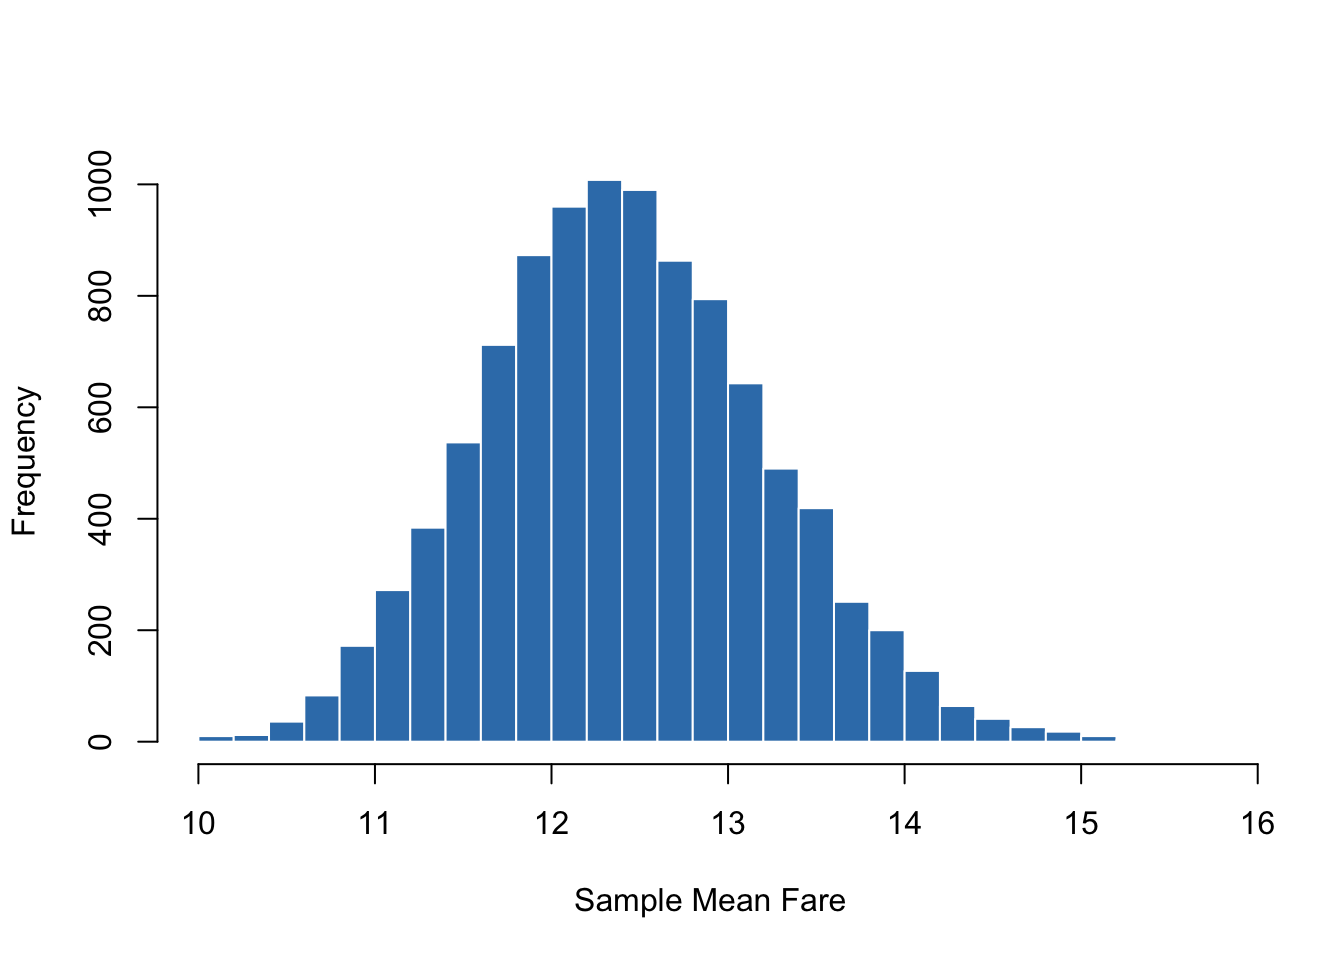
\includegraphics[width=\linewidth]{sampmean.png}

  \end{enumerate}

\end{solution}

\vfill

\newpage

\fullwidth{\section*{Confidence Intervals}}
\question You can consider the dataset of 162,997 taxi fares to be a sample
from a larger population. 

\begin{parts}
  
  \part What are some reasonable choices for this population?

  \begin{solution}
    One reasonable choice is the taxi fares for all 2013 New York City taxi
    trips.
  \end{solution}

  \vfill

  \part Give a range of plausible values for the mean of the population you
  specified in part~(a). \\
  \emph{Hint: you do not know $\sigma$ exactly, but since $n$ is large, you can
    assume $\sigma \approx s$.}

  \begin{solution}
    We can be 95\% confident that the population mean is within
    $2 \frac{\sigma}{\sqrt{n}}$ of the sample mean, where $n = 162997$.
    Using the approximation
    $\sigma \approx s$, we can get a 95\% confidence interval for the
    population mean:
    \begin{align*}
      \bar x \pm 2 \frac{s}{\sqrt{n}}
      &= (12.424) \pm 2 \frac{(7.966)}{\sqrt{162997}} \\
      &= 12.424 \pm 0.039 \\
      &= (12.385, 12.463)
    \end{align*}
  \end{solution}

  \vfill

  \part Under what conditions will your ``range of plausible values'' be
  trustworthy?

  \begin{solution}
    Since the sample size is large ($n = 162997$), the
    the Central Limit Theorem will be in force---making our confidence interval
    trustworthy---as long as the samples are drawn independently from the
    population. This will be the case if the sample is a simple random sample
    from the population. 

    If there is any bias in the sampling procedure, for example if the
    sample contains a disproportionate number of weekend trips, then the
    interval will not be valid.
  \end{solution}

  \vfill

\end{parts}
\newpage

\end{questions}

\end{document}
